% This is not necessarily in the format for a VUW thesis chapter.


%Finished July 19, 2013

\documentclass[a4paper]{report}

\usepackage{amssymb, amsmath}
\usepackage{tikz}
\usetikzlibrary{calc}

\usepackage{marvosym}


\title{Chapter 3: The Mathematical Model}
\author{Nat Lund}

\newcommand{\beff}{\ensuremath{b_{\mathrm{eff}}}}
\newcommand{\bhigh}{\ensuremath{b_{\mathrm{high}}}}
\newcommand{\blow}{\ensuremath{b_{\mathrm{low}}}}
\newcommand{\phislip}{\ensuremath{\phi_{\mathrm{slip}}}}
\newcommand{\phisol}{\ensuremath{\phi_{\mathrm{solid}}}}
\newcommand{\sigsol}{\ensuremath{\sigma_{\mathrm{solid}}}}
\newcommand{\gamsol}{\ensuremath{ \dot{\gamma}_{\mathrm{solid}} }} 

\newcommand{\sep}{\begin{equation*} \star \end{equation*}}

\begin{document}
\maketitle

We shall now derive an expression for the effective slip length of a rough, mixed-slip surface.  To begin, we translate the physical problem into the precise language of mathematics.  That is, we construct a mathematical model that maps to the essential features of physical reality.

A mathematical object that figures prominently in the model is the Fr\'{e}chet derivative.  To avoid cluttering the exposition later, we recall its features here.


\subsection*{Mathematical Preliminary: The Fr\'{e}chet Derivative}


The differing needs of the maths, physics and engineering communities can cause irritating inconsistencies in notation and nomenclature.  Being at the intersection of maths, physics and engineering, fluid mechanics is particularly prone to this.  Thus, it is necessary to define terms before ploughing into the derivation.  Disclaimer: the following language and notation may not be `standard', but they follow the conventions of the (rigorous) textbooks of C. Pozrikidis \cite{Pozrikidis1997, Pozrikidis2001}.

%Disclaimer: the following language and notation are not necessarily `standard' in any sense; they %reflect the ad hoc nature of my own education in mathematical physics, and their expediency for solving %a specific problem in this thesis.

The Fr\'{e}chet derivative is a generalization of the familiar derivative of a function of one real variable, to the more abstract `functions on Banach spaces'.  Happily, for finite-dimensional spaces, it is in fact the Jacobian matrix.

Consider a vector field in $\mathbb{R}^2$, with Cartesian coordinates.  At each point $x,y$ in space there is a vector $\vec{u} = (u,v)$, with $u$ and $v$ depending on $x$ and $y$ so that $\vec{u} = (u(x,y),v(x,y))$.  Then $\vec{u}$ can be considered a vector valued function on $\mathbb{R}^2$, with Jacobian matrix:

\begin{equation}
D \vec{u} = 
\begin{bmatrix}
\frac{\partial u}{\partial x} & \frac{\partial u}{\partial y} \\
\frac{\partial v}{\partial x} & \frac{\partial v}{\partial y}
\end{bmatrix}
=
\begin{bmatrix}
\partial_x u & \partial_y u \\
\partial_x v & \partial_y v
\end{bmatrix}
\end{equation}


The Fr\'{e}chet derivative is a \emph{spatial} derivative of a vector.  It gives the change in a vector field as one moves from point $\vec{x_0} = (x_0,y_0)$ in the direction $\vec{a}$.
The vector at point $\vec{x}_0$ is $\vec{u}(\vec{x}_0)$.  What is the vector at a point a short distance $\vec{a}$ away?  It is approximately $\vec{u}(\vec{x}_0)$ plus a correction $ D \vec{u} \cdot \vec{a}$ that depends on $\vec{a}$:

\begin{equation}
\vec{u}(\vec{x}_0 + \vec{a}) \simeq \vec{u}(\vec{x}_0) + D \vec{u} \cdot \vec{a}
\end{equation}

The approximation becomes exact as the magnitude of $\vec{a}$ tends to zero.

\begin{center}
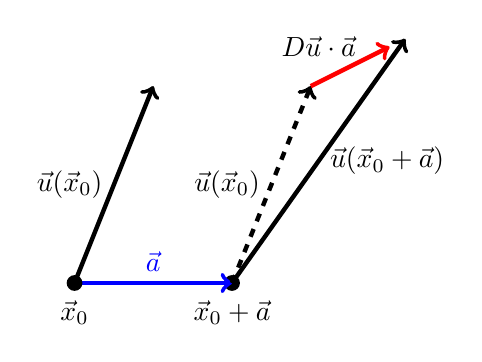
\begin{tikzpicture}
\draw[->,ultra thick] (0,0) -- node[left]{$\vec{u}(\vec{x}_0)$} (1,2.5);

\fill (2,0) circle (1mm);
\node at (2,-0.1) [below] {$\vec{x}_0 + \vec{a} $};
\draw[->,ultra thick,color=blue] (0,0) -- node[above]{$\vec{a}$} (2,0);
\fill (0,0) circle (1mm);
\node at (0,-0.1) [below] {$\vec{x}_0 $};

\draw[->,ultra thick,dashed] (2,0) -- node[left]{$\vec{u}(\vec{x}_0)$} +(1,2.5);
\draw[->,ultra thick,color=red] (2,0) ++(1,2.5) -- ++(1,0.5);
\node at (3.1,3) {$D \vec{u} \cdot \vec{a}$};

\draw[->,ultra thick] (2,0) -- node[right]{$\vec{u}(\vec{x}_0 + \vec{a})$} ++(2.2,3.1);

\end{tikzpicture}
\end{center}

The correction vector $ D\vec{u} \cdot \vec{a}$ is the tensor dot product of the Fr\'{e}chet derivative with the vector $\vec{a}$. The tensor dot product is defined as
\begin{equation}
\vec{b} = T \cdot \vec{a} ,\quad b_i = T_{ij} a_j
\end{equation}
which is the same as the familiar matrix multiplication of a vector:
\begin{equation}
D \vec{u} \cdot \vec{a} =
\begin{bmatrix}
\partial_x u & \partial_y u \\
\partial_x v & \partial_y v
\end{bmatrix}
\begin{bmatrix}
a_x \\ a_y
\end{bmatrix}
=
\begin{bmatrix}
(\partial_x u) a_x + (\partial_y u) a_y \\
(\partial_x v) a_x + (\partial_y v) a_y
\end{bmatrix}
\end{equation}

$ D\vec{u} \cdot \vec{a}$ is known as the directional derivative of $\vec{u}$ in the direction $\vec{a}$.

\subsubsection*{The Velocity Gradient Tensor}
If the vector field is a \emph{velocity} vector field $\vec{u}$, then it is convenient to work with the \textbf{velocity gradient tensor}, denoted $\nabla \vec{u}$.  This is the transpose of the Fr\'{e}chet derivative of the velocity field:
\begin{equation}
\nabla \vec{u} = D\vec{u}^T = 
\begin{bmatrix}
\partial_x u & \partial_x v \\
\partial_y u & \partial_y v
\end{bmatrix}
\end{equation}

This provides a linear approximation to the flow field in the vicinity of $\vec{x}_0$ via:
\begin{equation}
\vec{u}(\vec{x}) \simeq \vec{u}(\vec{x}_0) + (\vec{x} - \vec{x}_0)\cdot \nabla \vec{u}
\end{equation}

\vspace{1em}

\begin{center}
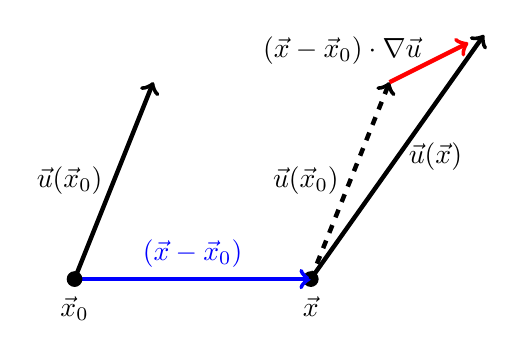
\begin{tikzpicture}
\draw[->,ultra thick] (0,0) -- node[left]{$\vec{u}(\vec{x}_0)$} (1,2.5);

\fill (3,0) circle (1mm);
\node at (3,-0.1) [below] {$\vec{x}$};
\draw[->,ultra thick,color=blue] (0,0) -- node[above]{$(\vec{x} - \vec{x}_0)$} (3,0);
\fill (0,0) circle (1mm);
\node at (0,-0.1) [below] {$\vec{x}_0 $};

\draw[->,ultra thick,dashed] (3,0) -- node[left]{$\vec{u}(\vec{x}_0)$} +(1,2.5);
\draw[->,ultra thick,color=red] (3,0) ++(1,2.5) -- ++(1,0.5);
\node at (3.4,2.9) {$ (\vec{x} - \vec{x}_0) \cdot \nabla \vec{u}$};

\draw[->,ultra thick] (3,0) -- node[right]{$\vec{u}(\vec{x})$} ++(2.2,3.1);

\end{tikzpicture}
\end{center}


An advantage of this convention is that the tensor dot product
\begin{equation}
\vec{b} = \vec{a} \cdot T = T^{T} \cdot \vec{a}, \quad b_i = a_j T_{ji}
\end{equation}
allows the notation to follow the form of the familiar one-dimensional case:
\begin{equation*}
f(x) \simeq f(x_0) + (x - x_0) \frac{df}{dx}
\end{equation*}


\vspace*{2em}
An interesting question: how does a vector change in the direction of \emph{the vector itself?} This vector `self gradient' looks like:

\begin{equation}
\vec{u} \cdot \nabla \vec{u}
=
\begin{bmatrix}
u & v
\end{bmatrix}
\begin{bmatrix}
\partial_x u & \partial_x v \\
\partial_y u & \partial_y v
\end{bmatrix}
=
\begin{bmatrix}
u \partial_x u + v \partial_y u \\
u \partial_x v + v \partial_y v
\end{bmatrix}
\end{equation}


Compare this with the \textbf{advection operator}  $(\vec{u} \cdot \nabla ) = u \partial_x + v \partial_y $, operating on vector $\vec{u}$:
\begin{equation}
(\vec{u} \cdot \nabla ) \vec{u} = ( u \partial_x + v \partial_y )
\begin{bmatrix}
u \\ v
\end{bmatrix}
=
\begin{bmatrix}
u \partial_x u + v \partial_y u \\
u \partial_x v + v \partial_y v
\end{bmatrix}
\end{equation}

We see that they are the same.  The advection operator usually appears in the derivation of the `material derivative'.  This alternative derivation via the velocity gradient tensor provides the useful intuition that the advection operator simply gives the change in a vector as one travels in \emph{the direction of the vector itself.} 


\section*{Modeling the Bulk Fluid: Navier Stokes}

A fluid mechanics problem starts with a bulk of fluid.  At each point in the fluid, the fluid has a velocity, thus, the fluid bulk is modeled as a vector field in 3-D space.  In diagrams, representative vectors appear as arrows, with the length of the arrow proportional to the magnitude of the vector.

\begin{center}
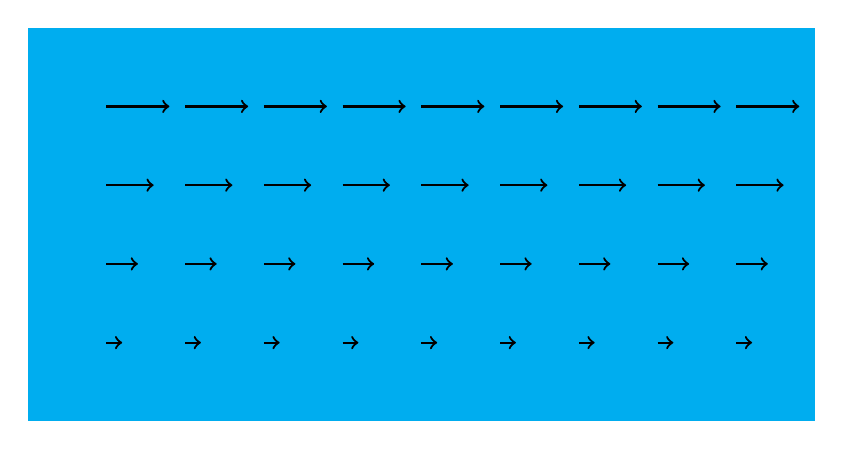
\begin{tikzpicture}

\fill[color=cyan] (0,0) rectangle (10,5);
\foreach \x in {1,2,3,4,5,6,7,8,9}
    \foreach \y in {1,2,3,4}
         \draw[->,thick](\x,\y) -- +(\y/5,0);

\end{tikzpicture}
\end{center}


\subsection*{Incompressible Liquid}

For a vector field, a \textbf{flux} can be defined.  If the fluid is an incompressible liquid, then the flux into a volume element will exactly equal the flux out of the volume element.  This is expressed in the model by stating that the vector quality of divergence is zero everywhere:
\begin{equation}
\nabla \cdot \vec{u} = 0
\end{equation}
This identity turns out to be extremely useful in making the ensuing mathematics tractable.



\subsection*{Viscous Newtonian Liquid}

An interesting fluid will also have other properties that hold at each point in the fluid: density, pressure, temperature.  Finally, truly exciting fluids have a \emph{viscosity} at each point, an `internal friction' that enables velocity to propagate through the fluid.  Viscosity is in fact the diffusion of momentum at the molecular level.
If the viscosity is constant throughout the fluid, and does not depend on velocity or velocity gradients, then the fluid is termed `Newtonian'. 

Viscosity acts with velocity gradients to produce \emph{forces} in the fluid.  An infinitesimal volume element in the fluid thus has a mass (density $\times$ volume) and experiences forces due to pressure and viscosity.  If we expect the laws of physics to hold in the fluid, then the volume element will obey Newton's second law $F= ma$.  This law is expressed as the Navier-Stokes equation.

If no other forces (eg. gravity) are relevant, and the fluid is \textbf{incompressible}, the Navier-Stokes equation is:

\begin{equation}
\rho \left( \frac{\partial \vec{u}}{\partial t} + (\vec{u}\cdot \nabla)\vec{u} \right) = -\nabla p +  \mu \nabla^2 \vec{u}
\end{equation}

If the equation is multiplied by the volume of the infinitesimal fluid element, then
the left-hand side is the acceleration, and the right-hand side is the force due to the pressure gradient and viscous shear.  The `advection operator'\\
 $(\vec{u} \cdot \nabla ) = u \partial_x + v \partial_y $
 gives the `inertial' term  $ (\vec{u}\cdot \nabla)\vec{u} $.

\section*{Microfluidics: Stokes or `creeping' flow}


The Navier-Stokes equations are believed to hold for all fluid flow.  However, the advection terms like $u \partial_x u$ in the differential equation are not linear, in the sense
that they cannot be put in the form $\dotsb + a_0 u + a_1 \partial_x u + \dotsb$.  Nonlinear partial differential equations are notoriously difficult to solve.  But there is hope.  In some physical cases, the nonlinear terms may be much smaller than the rest, and contribute only a negligible amount to the solution.  In that case, the nonlinear terms can be discarded, and the solution of the resulting linear equation is a very good approximation.  We will now show that this is true for the microfluidic case where slip effects are noticeable.

One clean way to compare the relative magnitudes of the terms is to nondimensionalize. The idea is this: express the fundamental physical quantities as fractions of a `characteristic' value. The fraction forms a new, dimensionless variable. Then typical values of the dimensionless variables have a magnitude on the order of one.  For example, consider Poiseuille flow down a straight pipe, where the average velocity is $U$.  The velocity $u$ varies from zero at the wall, to  $\frac{3}{2} U$ in the centre of the pipe.  Now define the dimensionless velocity $\hat{u} = u/U$.  Clearly, the magnitude of $\hat{u}$ will vary from zero at the wall, to $\frac{3}{2}$ in the centre. i.e. for most of the domain, $\hat{u}$ is `about one'.

A nondimensionalized equation will hopefully have many terms with a magnitude on the order of one, with the magnitude of the remaining terms easily evaluated.  Thus, nondimensionalizing expedites the process of deciding which terms are negligible enough to discard.

\subsubsection*{Example for Analysis: 2-D Poiseuille Flow}
This thesis analyses microfluidic flow experiments that reveal slip effects.  The canonical flow experiment is flow down a capillary --- a very thin pipe or channel.  
We shall use this type of flow to analyse our nondimensionalization.  For clarity, we shall stick to two dimensions; this models pressure-driven flow between two infinite flat planes separated by distance $L$.  This avoids messing about with cylindrical coordinates.  The solution is a parabolic velocity profile, the same Poiseuille flow as found in a straight, circular pipe.

The standard way to nondimensionalize pipe flow is to choose the pipe diameter $L$ as the characteristic length.  Likewise, we choose channnel width $L$, and average velocity $U$ as the characteristic velocity.


Then the nondimensional variables are:
\begin{equation}
\hat{x} = \frac{x}{L}, \quad \hat{y} = \frac{y}{L}, \quad
 \hat{u} = \frac{u}{U}, \quad \hat{v} = \frac{v}{U}
\end{equation}

The other variables are and pressure and time.  We would like to express them in terms of existing quantities.
It turns out that $ \mu U / L $ has units of pressure, and the ratio $L /U$ has units of time, so define characteristic pressure and time:
\begin{equation}
P = \frac{\mu U}{L}, \quad T = \frac{L}{U}
\end{equation}
giving dimensionless variables $\hat{p} = p/P$ and $\hat{t}=t/T$:
\begin{equation}
\hat{p} = \frac{L}{\mu U} p, \quad \hat{t} = \frac{U}{L}t
\end{equation}

Thus we can substitute
\begin{equation}
x = L\hat{x}, \quad y = L\hat{y}, \quad u = U \hat{u}, \quad v = U \hat{v}, 
\quad p = \frac{\mu U}{L}\hat{p}, \quad t = \frac{L}{U}\hat{t}
\end{equation}
into the Navier-Stokes equation.  For clarity, we focus on just the $x$ component:
\begin{equation}
\rho \left( \frac{\partial u}{\partial t} +
 u \frac{\partial u}{\partial x} + v\frac{\partial u}{\partial y} \right) =
 - \frac{\partial p}{\partial x} + 
\mu \left( \frac{\partial^2 u}{\partial x^2} + \frac{\partial^2 u}{\partial y^2} \right)
\end{equation}

Substitute:
\begin{equation}
\rho \left( \frac{\partial U\hat{u}}{\partial \frac{L}{U}\hat{t}} +
U\hat{u} \frac{\partial U\hat{u}}{\partial L\hat{x}} +
U\hat{v} \frac{\partial U\hat{u}}{\partial L\hat{y}} \right) =
 - \frac{\partial \frac{\mu U}{L} \hat{p}}{\partial L\hat{x}} + 
\mu \left( \frac{\partial^2 U\hat{u}}{\partial (L\hat{x})^2} + 
\frac{\partial^2 U\hat{u}}{\partial (L\hat{y})^2} \right)
\end{equation}

\begin{equation}
\rho \frac{U^2}{L} \left( \frac{\partial \hat{u}}{\partial \hat{t}} +
\hat{u} \frac{\partial \hat{u}}{\partial \hat{x}} +
\hat{v} \frac{\partial \hat{u}}{\partial \hat{y}} \right) =
 - \frac{\mu U}{L^2} \frac{\partial \hat{p}}{\partial \hat{x}} + 
\frac{\mu U}{L^2} \left( \frac{\partial^2 \hat{u}}{\partial \hat{x}^2} + 
\frac{\partial^2 \hat{u}}{\partial \hat{y}^2} \right)
\end{equation}

\begin{equation}
\text{Now multiply both sides by} \quad \frac{L^2}{\mu U}
\end{equation}

\begin{equation}
\frac{\rho L U}{\mu} \left( \frac{\partial \hat{u}}{\partial \hat{t}} +
\hat{u} \frac{\partial \hat{u}}{\partial \hat{x}} +
\hat{v} \frac{\partial \hat{u}}{\partial \hat{y}} \right) =
 -  \frac{\partial \hat{p}}{\partial \hat{x}} + 
\left( \frac{\partial^2 \hat{u}}{\partial \hat{x}^2} + 
\frac{\partial^2 \hat{u}}{\partial \hat{y}^2} \right)
\end{equation}


\vspace{1em}
Define Kinematic Viscosity
\begin{equation}
\nu = \frac{\mu}{\rho}
\end{equation}
Then define the \textbf{Reynolds Number:}
\begin{equation}
\mathrm{Re} = \frac{L U}{\nu}
\end{equation}

Thus the $x$ component of the Navier-Stokes equations are:
\begin{equation}
\mathrm{Re} \left( \frac{\partial \hat{u}}{\partial \hat{t}} +
\hat{u} \frac{\partial \hat{u}}{\partial \hat{x}} +
\hat{v} \frac{\partial \hat{u}}{\partial \hat{y}} \right) =
 -  \frac{\partial \hat{p}}{\partial \hat{x}} + 
\left( \frac{\partial^2 \hat{u}}{\partial \hat{x}^2} + 
\frac{\partial^2 \hat{u}}{\partial \hat{y}^2} \right)
\end{equation}


\vspace{1em}
We are now in a position to look at the relative magnitudes of the terms.

\subsubsection*{Magnitudes of Terms}

We will start with the terms containing the velocity.
\vspace{1em}

A typical capillary flow experiment is carried out with flow rates held constant. Therefore
\begin{equation}
\frac{\partial \hat{u}}{\partial \hat{t}} = 0
\end{equation}
For the purposes of our analysis, we shall assume that flow is steady, so this term vanishes.


%The characteristic time $T = L/U$ was chosen for dimensional convenience, not because it is a typical time scale.  It evaluates to
%\begin{equation}
%T = \frac{L}{U} = \frac{0.0001}{0.01} = 0.01 \;\; \text{seconds}
%\end{equation}
%
%Typically, for capillary flow experiments, velocity is constant, once equilibrium is reached. Thus, in general
%\begin{equation}
%\frac{\partial \hat{u}}{\partial \hat{t}} = 0
%\end{equation}
%In any case,  we can investigate how rapidly the velocity must change for this term to become significant:  If the characteristic velocity \emph{doubles}, and takes \emph{at least} 0.01 seconds to do so, then
%\begin{equation}
%\frac{\partial \hat{u}}{\partial \hat{t}} = \frac{1}{[\text{time} \geq 1]}\, \leq \, 1
%\end{equation}
%So if velocities in a microfluidic experiment change no quicker than doubling in 1/100th of a second, then the time-dependent term is at most of order one.  But typical capillary flow experiments involve steady flow, so this term vanishes.

\vspace{1em}
We have chosen Poiseuille flow to illustrate our nondimensionalization.  Since it has an exact solution, we know exactly what the velocity and its derivatives are.  With average velocity scaled to unity, and channel width also scaled to unity, the parabolic velocity profile looks like:

\begin{center}
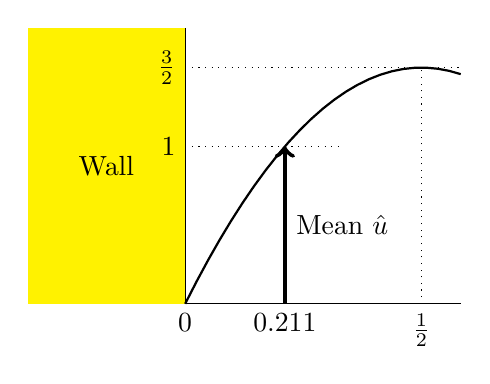
\begin{tikzpicture}
\fill [color=yellow] (0,0) rectangle node [color=black] {Wall}(-2,3.5);

\draw (0,0) -- (0,3.5);
\draw (0,0) -- (3.5,0);
\node at(0,0) [below] {0};
\draw [dotted] (3,0) -- ++(0,3);
\node at (3,0)[below] {$\frac{1}{2}$};
\draw [dotted] (0,2) -- ++ (2,0);
\node at (0,2)[left] {1};
\draw [dotted] (0,3) -- ++(3.5,0);
\node at (0,3) [left] {$\frac{3}{2}$};

\draw[thick] plot [domain = 0:3.5](\x, {3 - 0.3333*((\x - 3)^2)}  );

\draw[ultra thick,->] (1.266,0) -- node[right]{Mean $\hat{u}$} ++(0,2);
\node at (1.266,0) [below] {0.211};

\end{tikzpicture}
\end{center}


By construction, the $\hat{u}$ term ranges from zero to $\frac{3}{2}$. Hence, $\hat{u}$ is of order one.

For \emph{strict} Poiseuille flow, the walls are perfectly flat, and the velocity perpendicular to the wall is zero everywhere.  That is, $\hat{v} = 0$ always. 

But we may consider a channel with roughness on the walls, with the amplitude of the roughness \emph{small} compared to the channel width, so that the flow is Poiseuille-like.  Then, near the wall, the transverse velocity $\hat{v}$ may approach the magnitude of $\hat{u}$.  The magnitude of $\hat{u}$ near the wall is small compared to the average, so we would expect perhaps $\hat{v} < 0.1$.  That is, for rough-walled Poiseuille-like flow, $\hat{v}$ is of order 0.1, at most.

\vspace{1em}
For the parabolic flow profile of Poiseuille flow, the derivative of velocity is linear:
\begin{center}
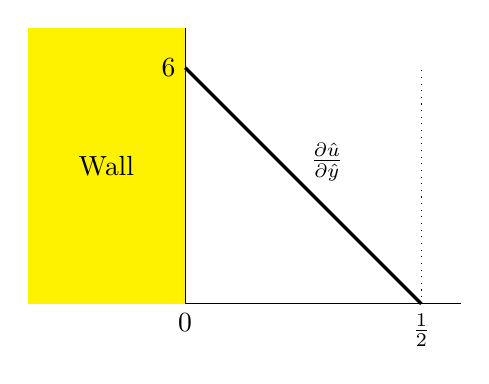
\begin{tikzpicture}
\fill [color=yellow] (0,0) rectangle node [color=black] {Wall}(-2,3.5);

\draw (0,0) -- (0,3.5);
\draw (0,0) -- (3.5,0);
\node at(0,0) [below] {0};
\node at (3,0)[below] {$\frac{1}{2}$};
\draw [dotted] (3,0) -- ++(0,3);

\node at (0,3) [left] {6};

\draw [very thick] (0,3) -- (3,0);
\node at (1.8,1.8) {$\frac{\partial \hat{u}}{\partial \hat{y}} $};

\end{tikzpicture}
\end{center}

The average \emph{value} of $\partial_y \hat{u}$ over the channel width is zero.  But the average \emph{magnitude} is 3.  In the tradition of theoretical physics, $\partial_{\hat{y}} \hat{u}$ is `of order one'.

For strict Poiseuille flow, $\hat{u}$ has no $x$-dependence, so $\partial_{\hat{x}} \hat{u} = 0$ everywhere.

For rough-walled Poiseuille-like flow, the wall corrugations will cause the $x$ velocity to change in the $x$ direction, over the period of the corrugation.  The roughness period must very small compared with the channel width for the flow to remain Poiseuille-like.  The $x$ velocity in the vicinity of the wall is on the order of 0.1, and varies by perhaps 10\% over the roughness period.  Thus, in the vicinity of the wall, $\partial_{\hat{x}} \hat{u} \sim (0.1 \times 0.1) / 0.01 = 1$.  But for the rest of the domain, the $x$ velocity will have vanishing $x$ dependence.  So \emph{average} $\partial_{\hat{x}} \hat{u}$ is more like 0.1.  Hence, $\partial_{\hat{x}} \hat{u}$ is of order 0.1.

\vspace{1em}
With $\hat{u}$ of order one and $\partial_{\hat{x}} \hat{u}$ of order 0.1, and $\hat{v}$ of order 0.1 and $\partial_{\hat{y}} \hat{u}$ of order one, the advection terms $\hat{u} \partial_{\hat{x}} \hat{u}$ and $\hat{v} \partial_{\hat{y}} \hat{u}$ are both of order 0.1.


\vspace{1em}
The second spatial derivative of the parabolic velocity profile is a constant:
\begin{center}
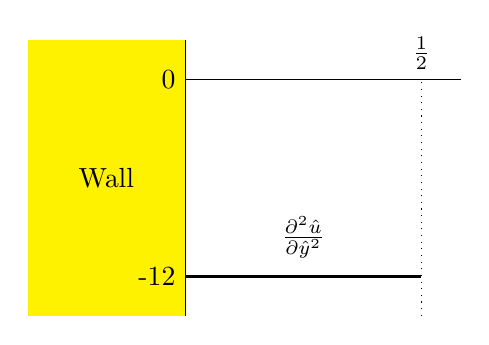
\begin{tikzpicture}
\fill [color=yellow] (0,0) rectangle node [color=black] {Wall}(-2,3.5);

\draw (0,0) -- ++(0,3.5);
\draw (0,3) -- ++(3.5,0);

\node at (3,3)[above] {$\frac{1}{2}$};
\draw [dotted] (3,0) -- ++(0,3);

\node at (0,3) [left] {0};

\node at (0,0.5) [left] {-12};
\draw [very thick] (0,0.5) -- ++(3,0);
\node at (1.5,1) {$\frac{\partial^2 \hat{u}}{\partial \hat{y}^2} $};

\end{tikzpicture}
\end{center}

For Poiseuille flow nondimensionalized in the standard way, $ \frac{\partial^2 \hat{u}}{\partial \hat{y}^2} = -12$.  That is, the magnitude is of order ten.

For strictly Poiseuille flow, the $x$ velocity has no $x$ dependence, so $\partial_{\hat{x}} \hat{u} = 0 $, and $ \partial^2_{\hat{x}} \hat{u} = 0 $.

For rough-walled Poiseuille-like flow, we have allowed that $\partial_{\hat{x}} \hat{u} \sim 1$ for the 10\% of the domain near the wall.  This reduces to near zero for the rest of the domain.  Therefore, $\partial_{\hat{x}} \hat{u}$ reduces from order one to zero in distance 0.1, hence average $ \partial^2_{\hat{x}} \hat{u}$ \emph{near the wall} is of order ten.  But it is zero over the rest of the domain, so the average over the channel is one.  Hence, $ \partial^2_{\hat{x}} \hat{u}$ is of order one.

\vspace{1em}
And now to the pressure term:  The characteristic pressure $P$ was chosen for dimensional convenience, not because it is necessarily a typical pressure.  So it is impossible to know the magnitude of $\hat{p}$ or $\partial_{\hat{x}} \hat{p}$.  But this doesn't matter; we have enough information to simplify, as we shall see.

\vspace{1em}
At this point, we can summarize what we know about the relative magnitudes of the terms in the Navier-Stokes equation.  For steady strict Poiseuille flow nondimensionalized in the standard way:
\begin{equation}
\mathrm{Re} \left( 
\underbrace{ \frac{\partial \hat{u}}{\partial \hat{t}} }_{\text{= 0}} +
\underbrace{ \hat{u} \frac{\partial \hat{u}}{\partial \hat{x}} }_{\text{= 0}} +
\underbrace{ \hat{v} \frac{\partial \hat{u}}{\partial \hat{y}} }_{\text{= 0}} 
\right) = 
\underbrace{ - \frac{\partial \hat{p}}{\partial \hat{x}} }_{\text{unknown}}
  + \left( 
\underbrace{ \frac{\partial^2 \hat{u}}{\partial \hat{x}^2} }_{\text{= 0}} + 
\underbrace{ \frac{\partial^2 \hat{u}}{\partial \hat{y}^2} }_{\sim 10} 
\right)
\end{equation}
Which simplifies considerably to:
\begin{equation}
0 = -  \frac{\partial \hat{p}}{\partial \hat{x}} + 
\left( \frac{\partial^2 \hat{u}}{\partial \hat{x}^2} + 
\frac{\partial^2 \hat{u}}{\partial \hat{y}^2} \right)
\end{equation}

But for rough-walled Poiseuille-like flow, things are not quite so simple:
\begin{equation}
\mathrm{Re} \left( 
\underbrace{ \frac{\partial \hat{u}}{\partial \hat{t}} }_{\text{= 0}} +
\underbrace{ \hat{u} \frac{\partial \hat{u}}{\partial \hat{x}} }_{\sim 0.1} +
\underbrace{ \hat{v} \frac{\partial \hat{u}}{\partial \hat{y}} }_{\sim 0.1} 
\right) = 
\underbrace{ - \frac{\partial \hat{p}}{\partial \hat{x}} }_{\text{unknown}}
  + \left( 
\underbrace{ \frac{\partial^2 \hat{u}}{\partial \hat{x}^2} }_{\sim 1} + 
\underbrace{ \frac{\partial^2 \hat{u}}{\partial \hat{y}^2} }_{\sim 10} 
\right)
\end{equation}

That is:
\begin{equation}
\mathrm{Re} \left( 
\underbrace{ \frac{\partial \hat{u}}{\partial \hat{t}}  +
     \hat{u} \frac{\partial \hat{u}}{\partial \hat{x}}  +
     \hat{v} \frac{\partial \hat{u}}{\partial \hat{y}} }_{\text{order 0.1}} 
\right) = 
\underbrace{ - \frac{\partial \hat{p}}{\partial \hat{x}}
 + \left( 
          \frac{\partial^2 \hat{u}}{\partial \hat{x}^2}  + 
          \frac{\partial^2 \hat{u}}{\partial \hat{y}^2}
  \right) }_{\text{order at least 10}}
\end{equation}

Importantly, we have discovered the relative magnitudes of the terms that \emph{do not depend on the physical situation.}  The above relation holds for Poiseuille flow of \emph{any} fluid at \emph{any} scale.  The parameters pertaining to the specific physical system are wrapped up into the Reynolds number.

Now is a good time, then, to evaluate the Reynolds number for the kind of microfluidic slip experiments we are considering.

\subsubsection*{Reynolds number for microfluidic channels}

A recent Poiseuille-type microfluidic slip experiment appears in the 2006 paper by Huang \emph{et al} in the Journal of Fluid Mechanics \cite{Huang2006}.  They looked at steady flow in channels 50 $\mu$m deep and 250 $\mu$m wide.  Particle velocimetry techniques showed a velocity distribution with a maximum velocity of about 600 $\mu$m s$^{-1}$.
When defining the Reynolds number for flow in a rectangular duct, the standard characteristic length to use is the \textbf{hydraulic diameter}, which is four times the cross-sectional area divided by the perimeter.  In this case it is 83.33 $\mu$m.
%$(4 \times 50 \times 250) / (50 + 250 + 50 + 250)$ which is 83.33 $\mu$m.

The viscosity of water at room temperatures is very close to $\mu = 0.001$ kgs$^{-1}$m$^{-1}$.  The density of water is $\rho = 1000$ kgm$^{-3}$.  We shall choose $L = 100 \mu$m and $U = 400 \mu$m s$^{-1}$ as conservative characteristic length and velocity scales.
Hence the Reynolds number evaluates to:
\begin{equation}
\mathrm{Re} = \frac{\rho L U}{\mu} = \frac{1000 \times 0.0001 \times 0.004}{0.001} = 0.4
\end{equation}
In the tradition of theoretical physics, this may be described as `of order 0.1'.
Thus the magnitudes of the two sides of the Navier-Stokes equation are:
\begin{equation}
\underbrace{
\mathrm{Re} \left( 
             \frac{\partial \hat{u}}{\partial \hat{t}}  +
     \hat{u} \frac{\partial \hat{u}}{\partial \hat{x}}  +
     \hat{v} \frac{\partial \hat{u}}{\partial \hat{y}} 
           \right)
}_{\text{order 0.04}}   = 
\underbrace{ - \frac{\partial \hat{p}}{\partial \hat{x}}
 + \left( 
          \frac{\partial^2 \hat{u}}{\partial \hat{x}^2}  + 
          \frac{\partial^2 \hat{u}}{\partial \hat{y}^2}
  \right) }_{\text{order at least 10}}
\end{equation}

So the right-hand side of the equation is \emph{at least} 250 times bigger than the left-hand side.  We have achieved our goal of finding which terms are negligible enough to discard.  We boldly make the tactical decision to throw away the left hand side, and solve instead the much simpler equation:
\begin{equation}
0 = -  \frac{\partial \hat{p}}{\partial \hat{x}} + 
\left( \frac{\partial^2 \hat{u}}{\partial \hat{x}^2} + 
\frac{\partial^2 \hat{u}}{\partial \hat{y}^2} \right)
\end{equation}

The $y$ component of the Navier-Stokes is:
\begin{equation}
\mathrm{Re} \left( 
\frac{\partial \hat{v}}{\partial \hat{t}} +
\hat{u} \frac{\partial \hat{v}}{\partial \hat{x}} +
\hat{v} \frac{\partial \hat{v}}{\partial \hat{y}}
 \right) =
    -  \frac{\partial \hat{p}}{\partial \hat{y}} + 
\left( \frac{\partial^2 \hat{v}}{\partial \hat{x}^2} + 
       \frac{\partial^2 \hat{v}}{\partial \hat{y}^2} 
\right)
\end{equation}
For pure Poiseuille flow, this reduces to 0 = 0.  For rough-walled Poiseuille-like flow, we expect $\hat{v}$ to be nonzero but very small compared to $\hat{u}$.  
So we anticipate no significant loss of information if we discard the left-hand side of the $y$ velocity equation.  If we do this, then we have simplified the Navier-Stokes vector equation to:
\begin{equation}
0 = -\hat{\nabla} \hat{p} + \hat{\nabla}^2 \hat{\vec{u}}
\end{equation}
or
\begin{equation}
\hat{\nabla}^2 \hat{\vec{u}} = \hat{\nabla} \hat{p}
\end{equation}
This is known as the Stokes equation, and describes very slow-moving flow described as `creeping' flow or Stokes flow.  Stokes flow is associated with Reynolds numbers Re $ \ll 1$.  Some perspective: for flow in a pipe, flows with Reynolds numbers below about 2,300 are always laminar, while flows with Reynolds numbers above about 4,000 are always turbulent.

In Stokes flow, the time-dependent and inertial terms are deemed to be negligible compared to the pressure and viscosity terms.  Thus, the Stokes equation describes the force balance between pressure and viscosity.

\subsubsection*{Redimensionalize back to Physical Units}

We will convert back into physical units. Substituting the definitions of the dimensionless variables back into the Stokes equation:
\begin{equation}
\left( \frac{\partial^2  \frac{u}{U}}{\partial (\frac{x}{L})^2} + 
\frac{\partial^2 \frac{u}{U}}{\partial (\frac{y}{L})^2} \right) =
\frac{\partial \frac{L}{\mu U} p}{\partial \frac{x}{L}}
\end{equation}

\begin{equation}
 \frac{L^2}{\mu U} \left( \frac{\partial^2 u}{\partial x^2} + 
\frac{\partial^2 u}{\partial y^2} \right) =
\frac{L^2}{\mu U}  \frac{\partial p}{\partial x}
\end{equation}

\begin{equation}
\text{Multiply both sides by} \quad \frac{\mu U}{L^2}
\end{equation}

\begin{equation}
\mu \left( \frac{\partial^2 u}{\partial x^2} + 
\frac{\partial^2 u}{\partial y^2} \right) =
\frac{\partial p}{\partial x}
\end{equation}

Similarly for the other vector components of the Stokes equation.

\vspace*{1em}
Thus, for microfluidic flow down a pipe, the bulk fluid obeys the Stokes equation:
\begin{equation}
\mu \nabla^2 \vec{u} = \nabla p
\end{equation}

In the field of microfluidics, it is customary to assume Stokes flow in all cases. However, we note that for example, the capillary slip experiment of Vinogradova 2009 \cite{Vinogradova2009} had velocities of up to 5 cm per second down a channel 100 $\mu$m wide, yielding a Reynolds number Re $\sim$ 1.  This makes the pressure and shear force terms only ten times larger than the inertial terms, so some error may be noticeable.
But, we shall follow the custom of microfluidics, and assume Stokes flow holds in the bulk.


%Vinogradova PRL 2009 had velocities up to 5 cm per second. Then Re = 1.  Too big.  Stokes %flow only sensible if Re $\ll$ 1.  Eg. Re $<$ 0.1.



\section*{Modeling the Boundary: Generalized Slip}
After establishing that the Stokes equation holds in the bulk fluid, we turn now to the boundary.  The first order of business is to define \emph{where} the boundary is.  As the discussion in Chapter 2 showed, there is some ambiguity about the location of the nominal boundary.  For a true physical surface, there may be a \emph{region} of finite width that could be labelled the `boundary'.  At the top of the region, the bulk fluid behaviour obtains, and at the bottom of the boundary, it is unambiguously solid.  

We are constructing a mathematical model of a physical system; in the model there will be a boundary that is a purely geometric surface (of zero width), and at any arbitrary distance above the boundary, the bulk fluid conditions will hold.  We need to decide exactly which part of the physical boundary region maps to our model boundary.  The sensible choice is: the top.

Here is why: As we descend down through the fluid towards the physical boundary, there will be a point at which the local conditions begin to deviate from that of the bulk.  Perhaps the density changes --- we are entering a `depletion region' with correspondingly lower viscosity.  In the mathematical model, there is a perfect distinction between `bulk' and `boundary'.  Thus we must identify the mathematical boundary with the very top of the physical boundary region.


\begin{center}
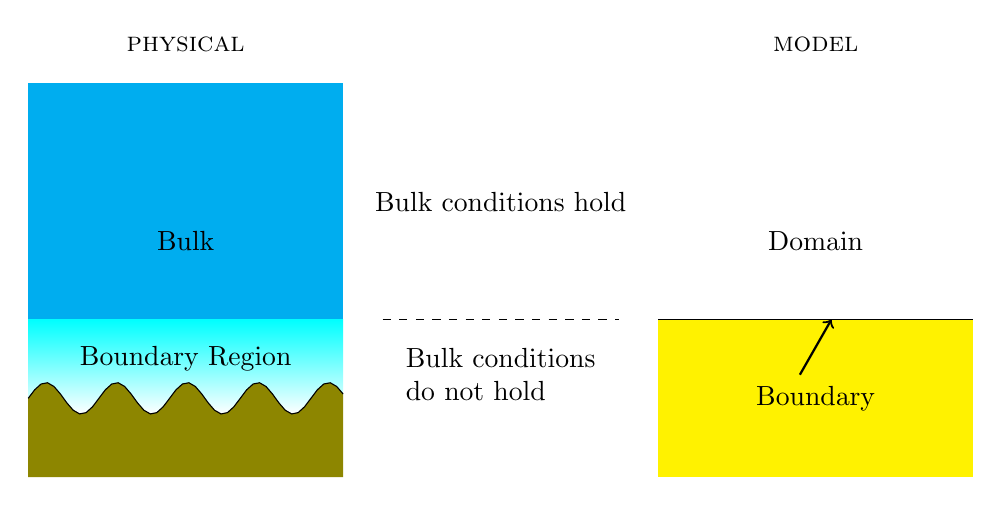
\begin{tikzpicture}
\fill[color=cyan] (0,0) rectangle (4,3);
\shade[top color=cyan](0,0) rectangle (4,-1.2);

\node at (2,1) {Bulk};
\node at (2,-0.5){Boundary Region};

\fill [color=olive,domain=0:4,samples=50] plot (\x,{ 0.2 * sin(7*\x r) - 1} ) -- (4,-2) -- ++(-4,0);
\draw [domain=0:4,samples=50] plot (\x,{ 0.2 * sin(7*\x r) - 1} );



\node at (6,1.5) {Bulk conditions hold};
\draw[dashed] (4.5,0) -- ++(3,0);
\node at (6,-0.7) [align=left]{Bulk conditions\\ do not hold};

\fill[color=yellow](8,0) rectangle ++(4,-2);
\draw(8,0) -- ++(4,0);
\node at (10,1) {Domain};
\node at (10,-1) {Boundary};
\draw[->,thick] (9.8,-0.7) -- (10.2,0);

\node at (2,3.5) {\textsc{physical}};
\node at (10,3.5) {\textsc{model}};

\end{tikzpicture}
\end{center}


\subsection*{Simple Shear with Navier Slip}

As explained in the introductory chapters, the classical boundary condition is `no slip', and the simplest extension to that is Navier slip, where the boundary velocity is proportional to the velocity gradient:
\begin{equation}
u_{\text{boundary}} = b \frac{\partial u}{\partial z} \bigg|_{\text{boundary}}
\end{equation}

This holds for a system exhibiting \textbf{simple shear:} a flat surface with laminar flow above it, with each lamina parallel to the boundary surface.  There is no velocity component normal to the surface.

\begin{center}
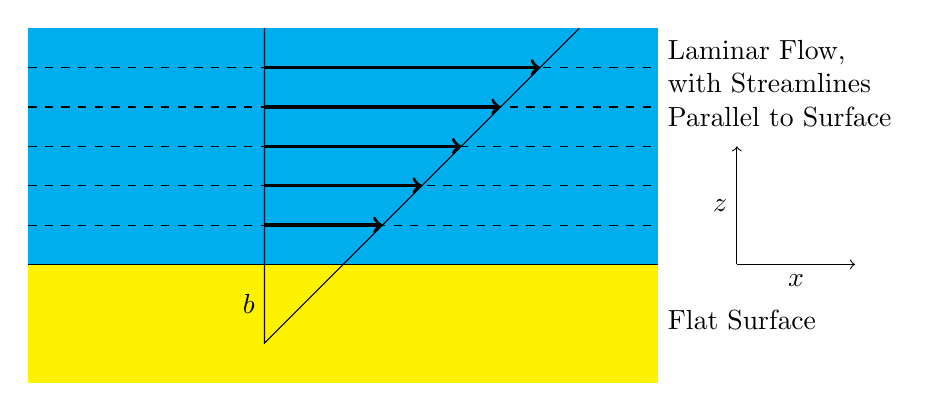
\begin{tikzpicture}
\fill[color=cyan] (-3,0) rectangle (5,3);
\fill [color=yellow] (-3,0) rectangle (5,-1.5);
\draw (-3,0) -- (5,0);
\foreach  \z in {0.5,1,...,2.5}
        {\draw[dashed] (-3,\z) -- ++(8,0);
         \draw[->, very thick](0,\z) -- ++(\z+1,0); };
\draw (0,3) -- (0,-1) -- ++(4,4);
\node at (0,-0.5)[left] {$b$};
\draw[->] (6,0) -- node[left] {$z$} ++(0,1.5);
\draw[->] (6,0) -- node[below] {$x$} ++(1.5,0);

\node at (5,-0.7)[right] {Flat Surface};
\node at (5,2.3) [right,align=left] {Laminar Flow,\\ with Streamlines\\Parallel to Surface};

\end{tikzpicture}
\end{center}

The laminae \emph{shear} past each other, giving rise to the viscous force.  The \emph{shear rate} is simply the velocity gradient: the rate of change of (parallel) velocity as we move in the normal direction.

The shear rate has an intuitive physical meaning.  Consider the action of simple shear on an infinitesimal cube of fluid: the cube starts with all sides at right angles, and is deformed into a parallelipiped.  The internal angle $\theta$ starts at $90^{\circ}$ and gets smaller.  In timeslice $\Delta t$ the change in angle $\Delta \theta$ looks like:

\begin{center}
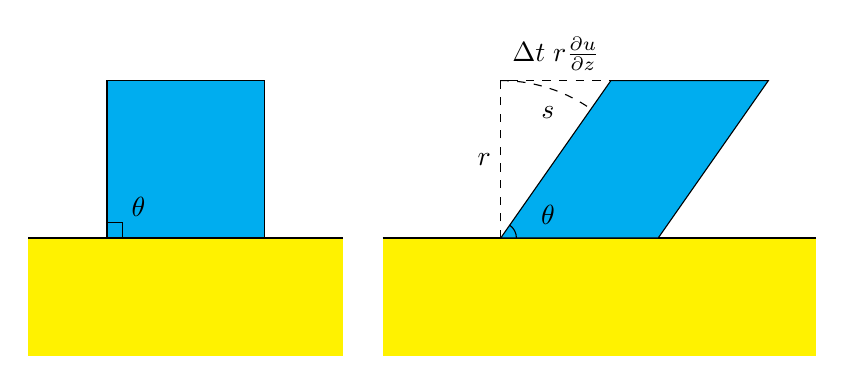
\begin{tikzpicture}

\fill[color=yellow] (-1,0) rectangle ++(4,-1.5);
\draw (-1,0) -- ++(4,0);
\draw[fill=cyan] (0,0) rectangle ++(2,2);
\draw (0.2,0) -- ++(0,0.2) -- ++(-0.2,0);
\node at (0.4,0.4) {$\theta $};


\fill[color=yellow] (3.5,0) rectangle ++(5.5,-1.5);
\draw (3.5,0) -- ++(5.5,0);
\draw[fill=cyan] (5,0) -- ++(1.4,2) -- ++(2,0) -- ++(-1.4,-2) -- ++(-2,0);

\draw[dashed] (5,0) -- node[left]{$r$} ++(0,2) -- node [above]{$\Delta t \; r \frac{\partial u}{\partial z}$} ++(1.4,0);
\draw[dashed] (5,2) arc (90:55:2cm);
\node at (5.6,1.6) {$s$};

\draw (5.2,0) arc (0:55:0.2cm);
\node at (5.6,0.3) {$ \theta$};

\end{tikzpicture}
\end{center}

In timeslice $\Delta t$, the top of the cube moves distance $\Delta t \, r \partial_z u$, and the angle changes by $\Delta \theta = s/r$.  For sufficiently small $\Delta t$, $s$ is much smaller than $r$, and $s \simeq \Delta t \, r \partial_y u$, so that $\Delta \theta \simeq \Delta t \, \partial_z u$.  In the limit $\Delta t \rightarrow 0$:

\begin{equation}
\text{shear rate} = \frac{d \theta}{d t} = \frac{\partial u}{\partial z}
\end{equation}


\subsection*{Oblique Shear and the Velocity Gradient Tensor}
If the surface is still flat, but \textbf{not} oriented such that the surface maps nicely to the plane $z=0$, then the shear rate must be defined with vector derivatives.

\begin{center}
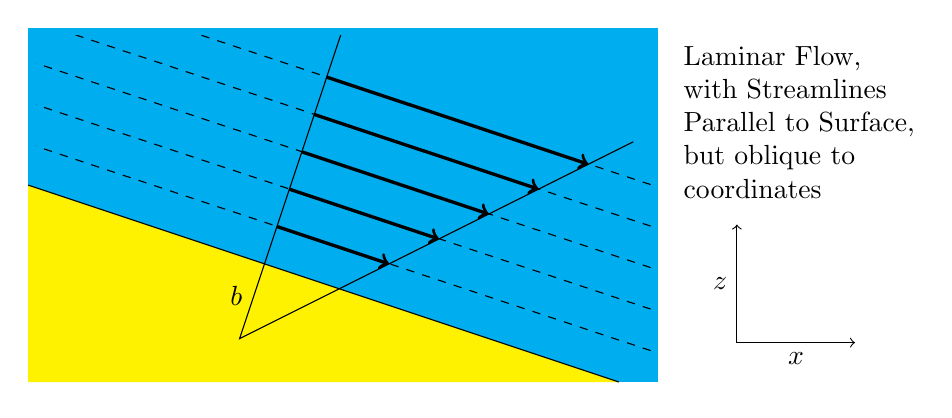
\begin{tikzpicture}
\fill[color=cyan] (-3,-1.5) rectangle (5,3);
\fill [color=yellow] (-3,-1.5) -- (-3,1) -- (4.5,-1.5);
\draw (-3,1) -- (4.5,-1.5);

\draw[->] (6,-1) -- node[left] {$z$} ++(0,1.5);
\draw[->] (6,-1) -- node[below] {$x$} ++(1.5,0);

%\node at (5,-0.7)[right] {Flat Surface};
\node at (5.2,1.8) [right,align=left] {Laminar Flow,\\ with Streamlines\\Parallel to Surface,\\but oblique to\\coordinates};

\clip (-2.9,-1.6) rectangle ++(8,4.5);
\foreach  \z in {0.5,1,...,2.5}
        {\draw[dashed] (-3,\z*1.054 + 1) -- ++(8,-2.66);
         \draw[->, very thick](0.316*\z, 0.949* \z) --
          ++(0.949*\z + 0.949,- 0.316*\z - 0.316); };
\draw (1,3) -- (-.316,-0.949) -- ++(5,2.5);
\node at (-0.158,-0.4)[left] {$b$};
\end{tikzpicture}
\end{center}

We introduce the unit vectors normal and tangent to the surface, $\vec{n}$ and $\vec{t}$. Then the tangential component of velocity is $ \vec{u} \cdot \vec{t}$.  
Because the streamlines are parallel to the flat surface, $\vec{u}$ is parallel to $\vec{t}$, so that $\vec{u} \cdot \vec{t}$ is in fact the \emph{magnitude} of $\vec{u}$.

We can define the shear rate as the rate of change of the tangential velocity in the normal direction. That is, the tangential component of the directional derivative of velocity in the normal direction.
The directional derivative of the velocity in the normal direction is $ \vec{n} \cdot \nabla \vec{u} $, and its tangential component is $ \vec{n} \cdot \nabla \vec{u} \cdot \vec{t}$.

\begin{center}
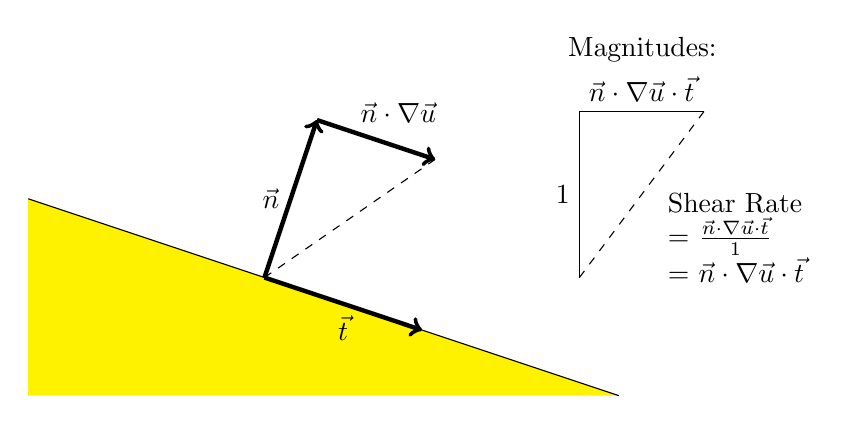
\begin{tikzpicture}
\fill[color=white] (-3,-1.5) rectangle (5,3);
\fill [color=yellow] (-3,-1.5) -- (-3,1) -- (4.5,-1.5);
\draw (-3,1) -- (4.5,-1.5);

%\draw[->] (6,-1) -- node[left] {$z$} ++(0,1.5);
%\draw[->] (6,-1) -- node[below] {$x$} ++(1.5,0);

\draw[ultra thick, ->] (0,0) -- node[left]{$\vec{n}$} (0.667,2);
\draw[ultra thick, ->] (0,0) -- node[below]{$\vec{t}$} (2,-0.667);

\draw[ultra thick, ->] (0.667,2) --  +(1.5,-0.5);
\node at (1.7,2.1) {$\vec{n} \cdot \nabla \vec{u}$};
\draw[dashed] (0,0) -- (2.167,1.5);

\draw (4,0) -- node[left]{1} ++(0,2.108) -- node[above]{$\vec{n} \cdot \nabla \vec{u} \cdot \vec{t}$} +(1.581,0);
\draw[dashed] (4,0) -- ++(1.581,2.108);

\node at (4.8,2.9) {Magnitudes:};
\node at (5,0.5)[right,align=left] {Shear Rate\\ = $\frac{\vec{n} \cdot \nabla \vec{u} \cdot \vec{t}}{1}$\\ = $ \vec{n} \cdot \nabla \vec{u} \cdot \vec{t}$};
\end{tikzpicture}
\end{center}

Thus for a \emph{flat} surface, with arbitrary coordinates, the shear rate is
\begin{equation}
\vec{n} \cdot \nabla \vec{u} \cdot \vec{t}
\end{equation}


\subsection*{Arbitrary Curved Surface and Deformation Rate Tensor}

But what if the surface is not flat?


\begin{center}
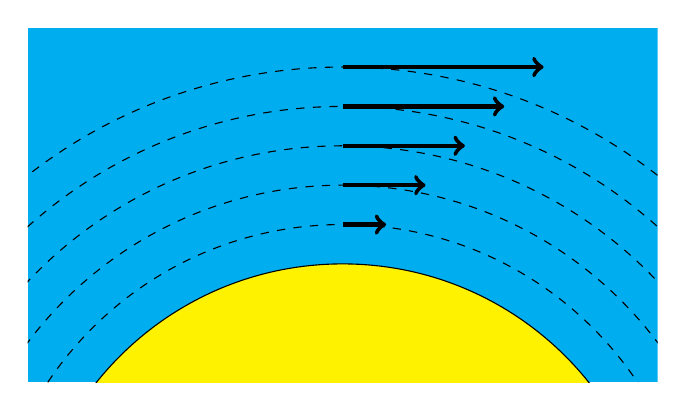
\begin{tikzpicture}
\clip (-4,-1.5) rectangle (4,3);
\fill[color=cyan] (-4,-1.5) rectangle (4,3);
\draw[fill=yellow] (0,-4) circle (4cm);

\foreach \k in {0.5cm,1cm,1.5cm,2cm,2.5cm}
           {
           \draw[dashed] (0,-4) circle (4cm + \k);
           \draw[ultra thick, ->] (0,\k) -- ++( 1.5 + \k,0);
           }



%\draw[fill=cyan] (0,0) rectangle ++(2,2);

\end{tikzpicture}
\end{center}

It is tempting to assume the shear rate is the same as in the case of the generalized flat surface:

\begin{center}
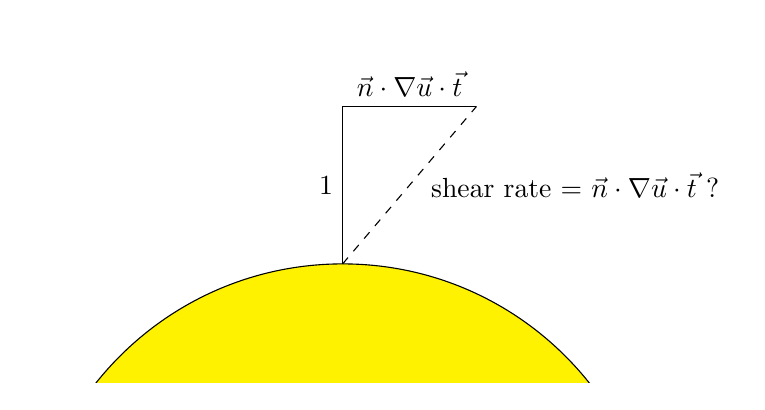
\begin{tikzpicture}
\clip (-4,-1.5) rectangle (5,3);

\draw[fill=yellow] (0,-4) circle (4cm);

\draw (0,0) -- node[left]{1}  ++(0,2) -- node[above] {$ \vec{n} \cdot \nabla \vec{u} \cdot \vec{t}$} ++(1.7,0);
\draw[dashed] (0,0) -- ++(1.7,2);

\node at (1,1)[right] {shear rate = $ \vec{n} \cdot \nabla \vec{u} \cdot \vec{t}$ ?};

\end{tikzpicture}
\end{center}

But consider the following \emph{possible} action on an infinitesimal cube of fluid:
\begin{center}
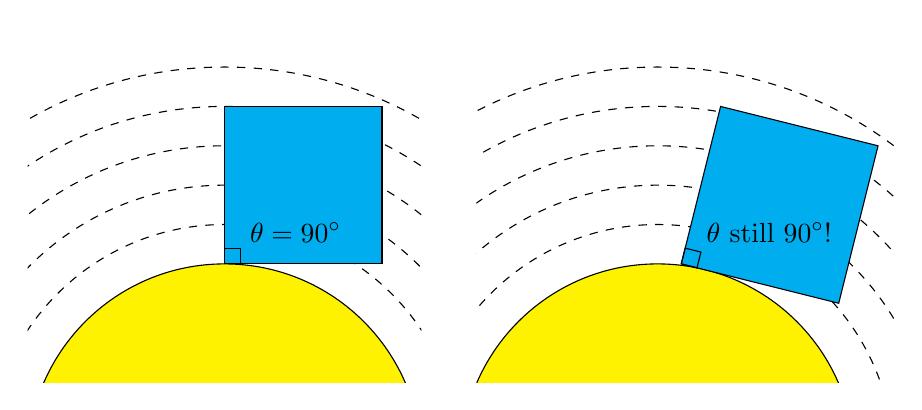
\begin{tikzpicture}
\begin{scope}
    \clip (-2.5,-1.5) rectangle (2.5,3);

    \foreach \k in {0.5cm, 1cm, 1.5cm,2cm,2.5cm}
              {
              \draw[dashed] (0,-2.5) circle (2.5cm + \k);
              }
    \draw[fill=yellow] (0,-2.5) circle (2.5cm);
\end{scope}

\draw[fill=cyan] (0,0) rectangle ++(2,2);
\draw (0.2,0) |- (0,0.2);

\node at (0.2,0.4)[right] {$\theta = 90^{\circ}$};


\clip (3.2,-1.5) rectangle (8.5,3);

\foreach \k in {0.5cm, 1cm, 1.5cm,2cm,2.5cm}
              {
              \draw[dashed] (5.5,-2.5) circle (2.5cm + \k);
              }

\draw[fill=yellow] (5.5,-2.5) circle (2.5cm);
\draw[fill=cyan] (5.8,0) -- ++(0.5,2)-- ++(2,-0.5) --++(-0.5,-2) -- ++(-2,0.5);
\draw (5.8,0) -- ++(0.05,0.2) -- ++(0.2,-0.05) -- ++(-0.05,-0.2) -- ++(-0.2,0.05);

\node at (6,0.4)[right] {$\theta$ still $90^{\circ}$!};

\end{tikzpicture}
\end{center}

The infinitesimal cubical element has \emph{rotated} (and perhaps translated) but \emph{not deformed.}
The laminae have \emph{not} slid past each other, and the cube has not been subjected to shear.  There will be no viscous stress operating within the cube.

In this case, $ \vec{n} \cdot \nabla \vec{u} \cdot \vec{t}$ is not the shear rate of the cube, but the rate of rotation (angular velocity).  To get the true shear rate, we need to somehow remove the rotation.

The velocity gradient tensor (and Fr\'{e}chet derivative) \emph{linearize} the flow field. $\nabla \vec{u}$ is a linear transformation of a direction vector (the result being the correction vector).  Geometrically, a linear transformation can be decomposed into a rotation, an area-preserving deformation, and an expansion.  Following the exposition in the texbook of C. Pozrikidis:

\begin{equation}
\nabla \vec{u} = \mathbf{\Xi} + \mathbf{E} + \frac{1}{2} (\nabla \cdot \vec{u})  \mathbf{I}
\end{equation}

The rotation is represented in the \textbf{vorticity tensor}, $\mathbf{\Xi}$, the deformation in the \textbf{deformation rate tensor}, $\mathbf{E}$, and the expansion in $ \frac{1}{2} (\nabla \cdot \vec{u}) \mathbf{I}$

Working, for clarity, with 2-dimensional flow only, the vorticity tensor is:
\begin{equation}
\mathbf{\Xi} = \frac{1}{2}(\nabla \vec{u} - \nabla \vec{u}^T) = 
\frac{1}{2}
\begin{bmatrix}
0  & \partial_x v - \partial_y u \\
\partial_y u - \partial_x v  & 0
\end{bmatrix}
\end{equation}

The deformation rate tensor is:
\begin{equation}
\mathbf{E} = \frac{1}{2}(\nabla \vec{u} + \nabla \vec{u}^T) - \frac{1}{2}(\nabla \cdot \vec{u}) \mathbf{I} = 
\frac{1}{2} 
\begin{bmatrix}
\partial_x u - \partial_y v  & \partial_x v + \partial_y u  \\
\partial_y u + \partial_x v  & \partial_y v - \partial_x u
\end{bmatrix}
\end{equation}

The expansion rate tensor is:
\begin{equation}
\frac{1}{2}(\nabla \cdot \vec{u}) \mathbf{I} =
\frac{1}{2}
\begin{bmatrix}
\partial_x u + \partial_y v  &  0  \\
0  &  \partial_x u + \partial_y v
\end{bmatrix}
\end{equation}

We will deal with liquids, which we assume to be incompressible.  Thus the divergence vanishes:
\begin{equation}
\nabla \cdot \vec{u} = 0
\end{equation}
Therefore, the expansion term vanishes, and the deformation rate tensor simplifies to:
\begin{equation}
\mathbf{E} = \frac{1}{2}(\nabla \vec{u} + \nabla \vec{u}^T) = 
\frac{1}{2}
\begin{bmatrix}
2 \partial_x u   & \partial_x v + \partial_y u  \\
\partial_y u + \partial_x v  &  2 \partial_y v
\end{bmatrix}
\end{equation}

So for incompressible fluids, the linearized flow field is fully described by two terms, the \emph{antisymmetric} and \emph{symmetric} parts of the velocity gradient tensor:
\begin{equation}
\nabla \vec{u} =
\frac{1}{2}(\nabla \vec{u} - \nabla \vec{u}^T) +
\frac{1}{2}(\nabla \vec{u} + \nabla \vec{u}^T) 
 = \mathbf{\Xi} + \mathbf{E}
\end{equation}

We have solved our problem: removing the rotational transforms from the velocity gradient tensor is as simple as $\nabla \vec{u} - \mathbf{\Xi} = \mathbf{E}$.  So the deformation rate tensor $\mathbf{E}$ contains all transformations of the velocity gradient tensor \emph{other} than rotation.  Specifically, it must describe all shear.

We illustrate this in a simple example of 2-dimensional flow, where the normal and tangent vectors happen to align with the coordinate axes:

\begin{center}
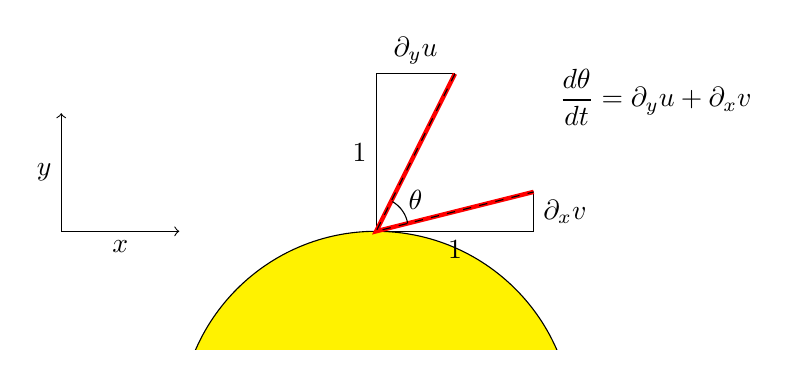
\begin{tikzpicture}
\everymath{\displaystyle}

\begin{scope}
    \clip (-2.5,-1.5) rectangle (2.5,1);
    \draw[fill=yellow] (0,-2.5) circle (2.5cm);
\end{scope}


\draw (0,0) -- node[left] {1} ++(0,2) -- node[above]{$\partial_y u $} ++(1,0);
\draw (0,0) -- node[below]{1} ++(2,0) -- node[right]{$\partial_x v$} ++(0,0.5);

\draw[color=red,ultra thick] (1,2)-- (0,0) -- (2,0.5);
\draw[dashed] (1,2) -- (0,0) -- (2,0.5);

\draw (0.4,0.1) arc (10:60:0.4cm);
\node at (0.5,0.4) {$\theta$};

\node at (2.2,1.7) [right] {$\frac{d\theta}{dt} = \partial_y u + \partial_x v$};

\draw[->] (-4,0) -- node[left] {$y$} ++(0,1.5);
\draw[->] (-4,0) -- node[below] {$x$} ++(1.5,0);

\end{tikzpicture}
\end{center}

We see that the true shear rate at this point is $\partial_y u + \partial_x v$. The normal and tangent vectors at this point are:
\begin{equation}
\vec{n} = 
\begin{bmatrix}
0 \\ 1
\end{bmatrix}
, \quad
\vec{t} =
\begin{bmatrix}
1 \\ 0
\end{bmatrix}
, \quad
\end{equation}
 What is $\vec{n} \cdot 2 \mathbf{E} \cdot \vec{t}$ ?
\begin{equation}
\vec{n} \cdot 2 \mathbf{E} \cdot \vec{t} = 
\begin{bmatrix}
0 \\ 1
\end{bmatrix}
\cdot
\begin{bmatrix}
2 \partial_x u   & \partial_x v + \partial_y u  \\
\partial_y u + \partial_x v  &  2 \partial_y v
\end{bmatrix}
\begin{bmatrix}
1 \\ 0
\end{bmatrix}
=
\partial_y u + \partial_x v
\end{equation}


We have intuitively confirmed that for a general fluid flow, the shear rate associated with an infinitesimal plane is:
\begin{equation}
\text{shear rate} = \frac{d\theta}{dt} = \vec{n} \cdot 2 \mathbf{E} \cdot \vec{t}
\end{equation}
where $\vec{n}$ and $\vec{t}$ are the unit normal and tangent vectors to the plane.

\subsubsection*{Generalized Slip Condition}

We have discovered the generalized shear rate: the rate of shear of an infinitesimal plane sliding over another infinitesimal plane.  If the plane is on the solid surface, then we can now write down a generalized Navier-type slip condition: the tangential velocity on the plane is proportional to the shear rate at the plane.  The constant of proportionality is of course the slip length $b$.

\begin{equation}
\vec{u} \cdot \vec{t} = b \; \vec{n} \cdot 2 \mathbf{E} \cdot \vec{t}
\end{equation}

Now $\mathbf{E}$ is symmetric, so $\vec{n} \cdot \mathbf{E} = \mathbf{E} \cdot \vec{n}$.  Furthermore, both sides of the equation are a dot product with $\vec{t}$, so we may simplify to:
\begin{equation}
\vec{u} = b \; 2 \mathbf{E} \cdot \vec{n}
\end{equation}

Or,
\begin{equation}
\vec{u} = b \, (\nabla \vec{u} + \nabla \vec{u}^T) \cdot \vec{n}
\end{equation}


\vspace{1em}

It remains only to note that the slip length is a \emph{function} of position, and that the boundary on which it holds is may also be described by a function. The boundary function will typically be a surface -- a `height' function $h(x,y)$ on the $x,y$ plane.

\section*{Complete Mathematical Model}

Our mathematical model can now be formally stated.  An bulk of fluid is situated above a boundary surface.  
The boundary surface is a function on the $x,y$ plane, and the $z$ direction is in general perpendicular to the boundary.

The fluid is an incompressible liquid, so the divergence is zero everywhere in the bulk:
\begin{equation}
\nabla \cdot \vec{u} = 0
\end{equation}

The liquid is Newtonian and the flow has a low Reynolds number, so flow at each point in the bulk obeys Stokes equation:
\begin{equation}
\mu \nabla^2 \vec{u} = \nabla p
\end{equation}
And fluid at each point on the boundary satisfies the generalized slip boundary condition:
\begin{equation}
\vec{u} = b \, (\nabla \vec{u} + \nabla \vec{u}^T) \cdot \vec{n}
\end{equation}


\vspace*{3em}
In the next chapter we shall find an expression for the effective slip by finding a \textbf{homogenized} solution to these partial differential equations.

%\begin{center} \vspace{3em} \Coffeecup \end{center}


\bibliography{Lund_Thesis.bib}
\bibliographystyle{plain}



\end{document}

TODO: clean up headings. Perhaps mention `directional derivative' and linearizing flow field in beginning.  Could also mention `vector gradient' and `tensor derivative' as meanings of $\nabla \vec{u}$, and `covariant derivative' as interpretation of $\nabla$.  But this seems unnecessary clutter.

 Maybe think about shear vector.  On second thoughts, no.  There is NO intuitive explanation of shear vector; I remember struggling with this 3 years ago.  Stress vector almost as bad.  Stress tensor is good for completeness, but unnecessary for this thesis. KISS.

\end{document}





